\section{Unsupervised Learning}

\subsection{k-Means Clustering}

Given an unlabelled dataset, we try to learn feature similarities based on proximity in feature space. Data points with similar features then should be grouped into the same cluster. k-Means tries to represent each cluster by a single (center) point $\mu_i$.

\begin{center}
	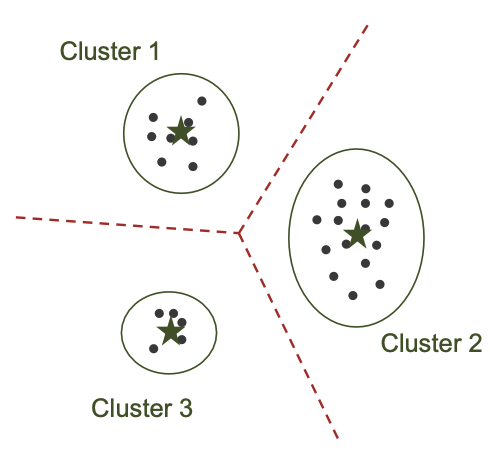
\includegraphics[width=0.6\columnwidth]{k-means.png}
\end{center}

Each data points is assigned by:
$$z_j = \argmin{i} ||x_j - \mu_i||_2, \quad z_j \in \{1, ..., k\}$$

To pick the optimal centers we try to minimize the sum of squared distances:
$$\hat{R} (\mu) = \sum_{i=1}^n \min_{j\in \{1,...,k\}} ||x_i - \mu_j||_2^2$$

This is a non-convex optimization problem and NP-hard. 

\columnbreak

One way of finding a good solution is Lloyd's heuristics:
\begin{enumerate}
	\item Initialize cluster centers $\mu^{(0)}$
	\item While not converged:
		\begin{enumerate}
			\item Assign each point to closest center:
				$$z_i \leftarrow \argmin{j\in \{1,...,k\}} ||x_i - \mu_j^{(t-1)}||_2$$		
			\item Update centers as mean of assigned data points:
				$$\mu_j^{(t)} \leftarrow \frac{1}{n_j} \sum_{i | z_i = j} x_i$$  	
		\end{enumerate}
\end{enumerate}

This guarantees to monotonically decrease the average squared distance in each iteration and converges to a local optimum. This local optimum is strongly dependent on the initialization. One way to initialize the centers is \textbf{k-Means++}:

\begin{enumerate}
	\item Start with random data point as center $\mu_1 = x_i$ where $i \sim \text{Unif}\{1,...,n\}$
	\item Add centers $2,...,k$ randomly, proportionally to the squared distance to closest selected center:
		$$\text{given } \mu_{1:j} \text{ pick } \mu_{j+1} = x_i$$ $$\text{ where } p(i) = \frac{1}{z} \min_{l \in \{1,...,j\}} ||x_i - \mu_l||_2^2$$
\end{enumerate}

To find the optimal number of clusters $k$ can not be done by cross-validation, as the loss keeps decreasing with larger $k$. We can either keep increasing $k$ until we reach a negligible decrease in loss or we can use regularization to add a penalty term for larger $k$.

\subsection{Principal Component Analysis}

PCA is used for dimensionality reduction. Given data $x_i \in \R^d$ we want to obtain a low-dimensional representation $z_i \in \R^k$ where $k < d$. One of the benefits of low-dimensional representation is that we can visualize data that we otherwise could not. Feature discovery is another use case for PCA, it can help us to discover features from data, e.g. Eigenfaces. We assume that our data is centered around the origin. 

Our goal is to learn the function $f(x) = Ax$ that maps the high dimensional data to the lower dimensions, while minimizing the reconstruction error. First we will look at the case $k = 1$.
$$\min_{w, z} \sum_{i=1}^n ||x_i - z_i w||_2^2 \quad \text{s.t. } ||w||_2 = 1$$

We limit $w$ to be of unit length to guarantee a unique solution.

\begin{center}
	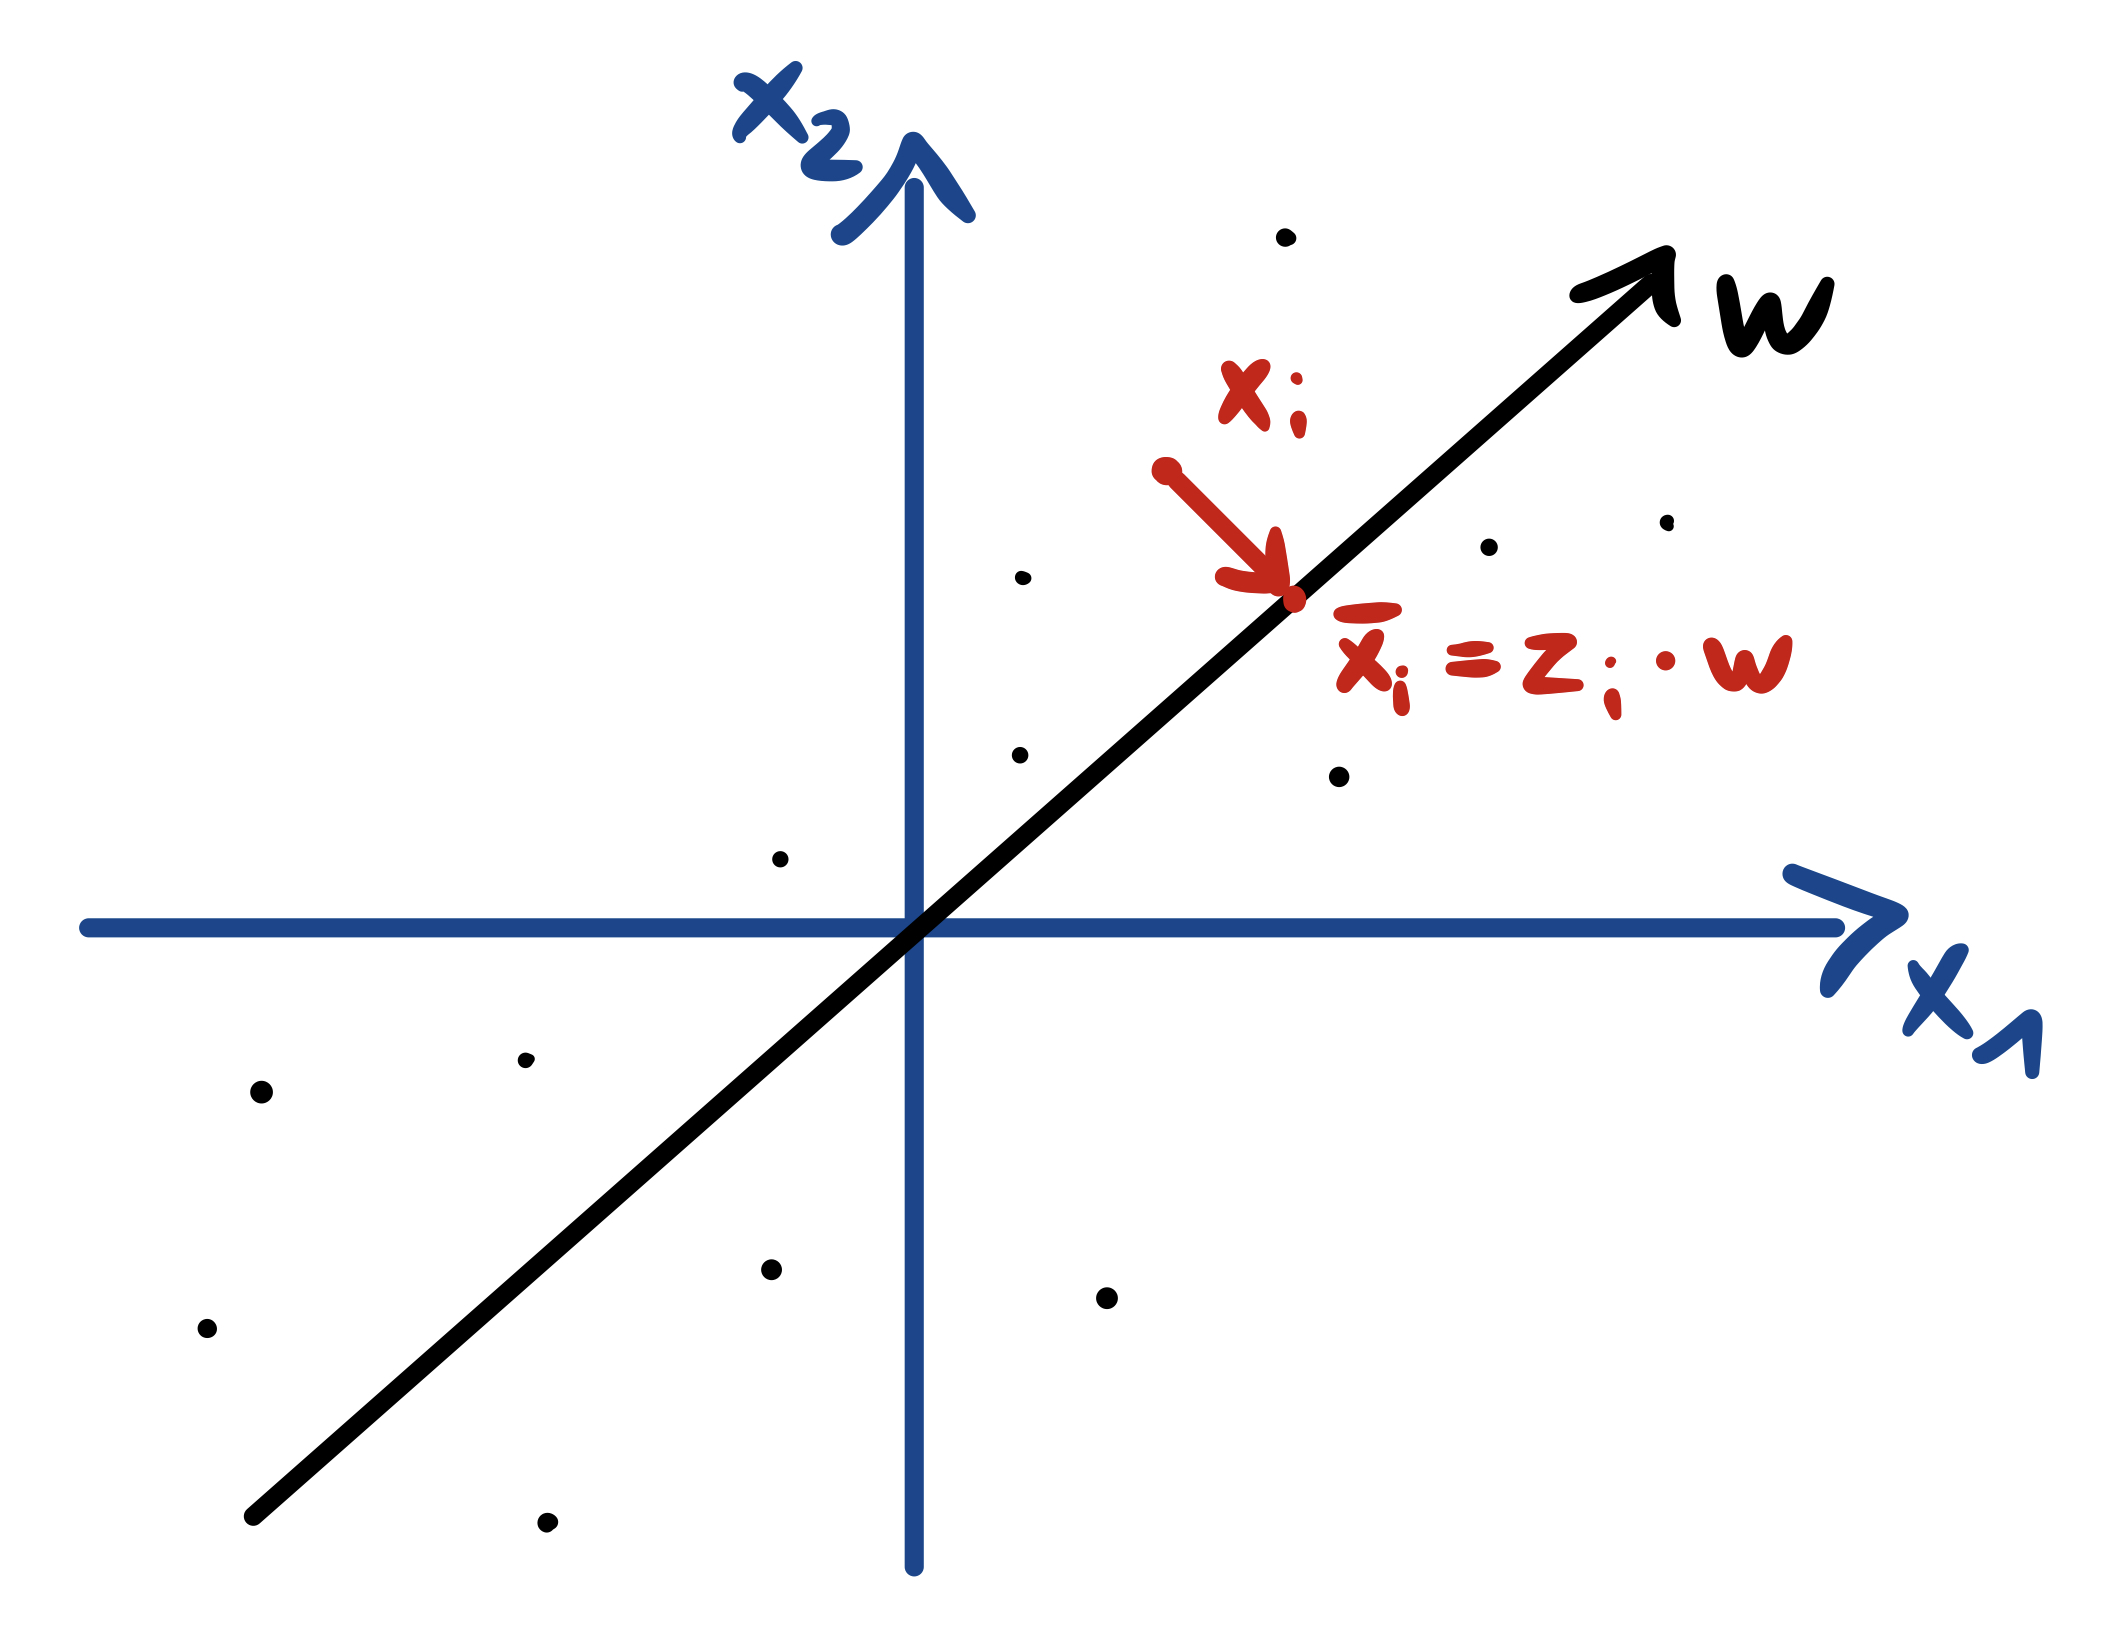
\includegraphics[width=0.7\linewidth]{pca.jpeg}
\end{center}

Since for a given $w$ the minimal distance vector $\bar{x}_i - x_i$ is perpendicular to $w$, we find that the optimal solution for $z_i = w^\top x_i$. We can now substitute $z_i$ and receive the following optimization goal:
$$\hat{w} = \argmin{||w||_2=1} \sum_{i=1}^n ||x_i - w w^\top x_i||_2^2$$

Which again can be reformulated as:
$$\hat{w} = \argmax{||w||_2=1} \; \sum_{i=1}^n (w^\top x_i)^2 \text{ or } \hat{w} = \argmax{||w||_2=1} \; w^\top \Sigma w$$

Where $\Sigma = \frac{1}{n} \sum_{i=1}^n x_i x_i^\top$ is the empirical covariance. Since we still have an argmax this is not a minimization problem anymore and we can not find a solution like in previous problems. There still exists a closed form solution given by the principal eigenvector of $\Sigma$, i.e. $w = v_1$ where for $\lambda_1 \geq ... \geq \lambda_d \geq 0$:
$$\Sigma = \sum_{i=1}^d \lambda_i v_i v_i^\top$$

Up until now everything was for $k = 1$. For $k > 1$ we have to change the normalization from $||w||_2 = 1$ to $W^\top W = I$ everything else is basically the same, we just take the first $k$ principal eigenvectors so that $W = [v_1, ..., v_k]$.

Choosing the optimal $k$ is different depending on our goal, for feature induction we use cross-validation else we often pick $k$ so that the variance of our data is mostly explained (other dimensions would add little information).

\subsubsection{PCA through SVD}

Another way of obtaining the PCA is through singular-value decomposition. Recall that we can represent any data matrix $X$ as $U S V^\top$ where $S$ is a diagonal matrix containing the singular values (singular values being the square root of eigenvalues). Now the top $k$ principal components are exactly the first $k$ columns of $V$.

\subsubsection{Kernel PCA}

Again we run into problems trying to work with complex arrangements of data, e.g. circles, swiss roll, etc.

\begin{center}
	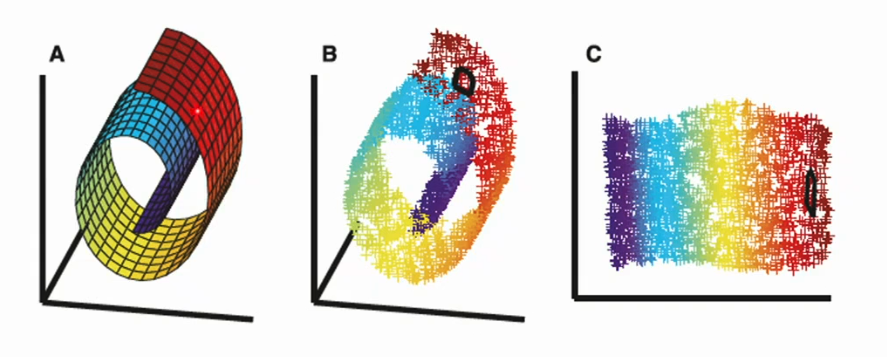
\includegraphics[width=\linewidth]{swiss-roll.png}
\end{center}

Similar to supervised learning where we worked with kernels, we can take the same approach for unsupervised learning. Since it holds $\Sigma = \frac{1}{n} \sum_{i=1}^n x_i x_i^\top = X^\top X$ we can apply the kernel trick. We start by assuming $w = \Phi^\top \alpha$, plugging this into our objective and the constraint we end up with:
$$\hat{\alpha} = \argmax{\alpha} \; \frac{\alpha^\top K^\top K \alpha}{\alpha^\top K \alpha}$$

We arrive at the general closed form solution:
$$\alpha^{(i)} = \frac{1}{\sqrt{\lambda_i}}v_i \quad K = \sum_{i = 1}^n \lambda_i v_i v_i^\top \quad \lambda_1 \geq ... \geq \lambda_n \geq 0$$

Given this, a new point $x$ is projected as $z$ where:
$$z_i = \sum_{j=1}^n \alpha_j^{(i)} k(x_j, x)$$

\subsection{Autoencoders}

Autoencoders are neural networks with a bottleneck layer and $d_{in} = d_{out}$. We want to minimize $\frac{1}{n}\sum_{i=1}^n ||x_i - \hat{x}_i||_2^2$. The idea is to learn the identity function:
$$\hat{x} = f(x; \theta) \text{ where } f(x; \theta) = f_{dec}(f_{enc}(x, \theta_{enc}); \theta_{dec})$$

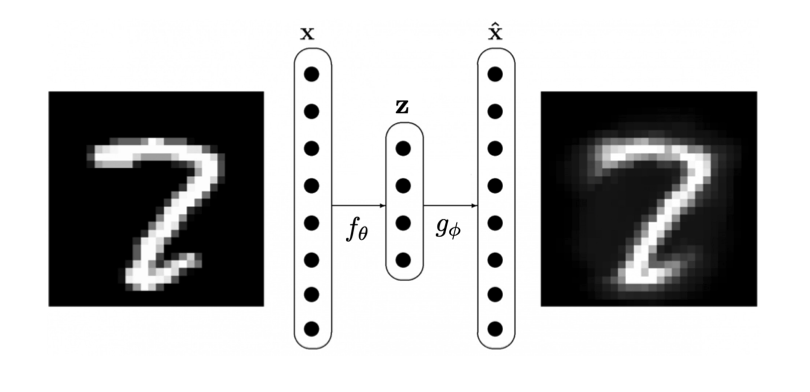
\includegraphics[width=\linewidth]{autoencoder.png}

If linear activation functions and the square loss between input and output are used, then the encoder learns PCA. Otherwise it learns some nonlinear embedding $z$ of the features.